\documentclass[se, manuscript]{copernicus}
\usepackage{mathptmx}


\begin{document}

\title{The impact of earthquake cycle variability on neotectonic and
paleoseismic slip rate estimates}

\Author[1, 2, 3]{Richard}{Styron}

\affil[1]{Earth Analysis, 21855 Bear Creek Road, Los Gatos, CA 95033 USA}
\affil[2]{Global Earthquake Model Foundation, Via Ferrata 1, Pavia 27100 Italy}
\affil[3]{Department of Geology, University of Kansas, Ritchie Hall, Earth Energy \& Environment Center, 1414 Naismith Drive,
Room 254, Lawrence, KS 66054 USA}

\runningtitle{Impact of earthquake cycle on slip rates}
\runningauthor{Richard Styron}
\correspondence{Richard Styron (richard.h.styron@gmail.com)}


\firstpage{1}
\maketitle

\begin{abstract}
Because of the natural variability (aleatoric uncertainty) in earthquake
recurrence intervals and coseismic displacements on a fault, cumulative
slip on a fault does not increase linearly or perfectly step-wise with
time; instead, some amount of variability in shorter-term slip rates
results. Though this variability could greatly affect the accuracy of
neotectonic (i.e., late Quaternary) and paleoseismic slip rate
estimates, these effects have not been quantified. In this study,
idealized faults with four different, representative earthquake
recurrence distributions are created with equal mean recurrence
intervals (1,000 years) and coseismic slip distributions, and the
variability in slip rate measurements over 500 to 100,000 year
measurement windows is calculated for all faults through Monte Carlo
simulations. The recurrence distributions used are quasi-periodic,
unclustered and clustered lognormal distributions, and an unclustered
exponential distribution. The results demonstrate that the most
important parameter is the coefficient of variation (\(COV\) = standard
deviation / mean) of the recurrence distributions rather than the shape
of the distribution itself. Slip rate variability over short time scales
(\textless{} 10,000 years or 10 mean earthquake cycles) is quite high,
but decreases with time and is close to stable after
\textasciitilde{}40,000 years (40 mean earthquake cycles). This
variability is higher for recurrence distributions with a higher
\(COV\). The natural variability in the slip rate estimates compared to
the true value is then used to estimate the epistemic uncertainty in a
single slip rate measurement (as one would make in a geological study)
in the absence of any measurement uncertainty. This epistemic
uncertainty is very high (a factor of 2 or more) for measurement windows
of a few mean earthquake cycles (as in a paleoseismic slip rate
estimate), but decreases rapidly to a factor of 1-2 with \textgreater{}5
mean earthquake cycles (as in a neotectonic slip rate study). These
uncertainties are independent of, and should be propagated with
uncertainties in fault displacement and geochronologic measurements used
to estimate slip rates. They may then aid in the comparison of slip
rates from different methods or the evaluation of potential slip rate
changes over time.
\end{abstract}

\introduction

Fault slip rates are generally estimated by dividing measurements of the
offset of geologic `marker' features by the time over which that offset
accumulated. The uncertainty in the resulting slip estimate is typically
treated as \emph{epistemic}, and quantified through the propagation of
the measurement uncertainties on the offset and time quantities
\citep[e.g.]{bird_uncertainties_2007,zechar_incorporating_2009}.
However, for slip rate estimates on active faults made from offset
measurements near the fault trace (i.e., within a horizontal distance
that is a small fraction of the fault's locking depth), the episodic
nature of surface displacement due to the earthquake cycle will
necessarily affect the results: If the measurements are taken
immediately before an earthquake, the measured offset and resulting slip
rate estimate will be lower than average, while if the measurements are
taken immediately after an earthquake, the offset and rate will be
higher.

The magnitude of the perturbation to the slip rate is, of course, a
function of the number of cumulative earthquakes that have contributed
to the measured offset. For older Quaternary markers that have
experienced tens to hundreds of major earthquakes, the effects will be
minor, and for bedrock geologic markers with kilometers of displacement,
the earthquake cycle is likely not worth accounting for. However, due to
progressive erosion of geologic markers and the challenge of dating many
late Pliocene to early Quaternary units (which are too old for
radiocarbon and many cosmogenic nuclide systems), geologists often have
no choice but to choose late Pleistocene to Holocene markers to date,
and these units may also be more desirable targets if the scientists are
primarily concerned with estimating the contemporary slip rate on a
fault with a slip rate that may vary over Quaternary timescales
\citep[e.g.]{rittase_temporal_2014,zinke_highly_2018}. For slow-moving
faults, the slip either long waiting to be released, or recently
released, may represent a sizeable fraction of the measured fault
offset.

Careful paleoseismologists and neotectonicists will take this into
account in their slip rate calculations if sufficient data are
available, especially in the years after a major earthquake
\citep[e.g.]{rizza_earthquake_2015}, and many others will discuss the
potential effects if the data are not \citep[e.g.]{lifton_latest_2015}.
These workers may only consider the time since the last earthquake,
often making the assumption (stated or not) that the earthquakes are
identical in slip and perfectly periodic.

However, the recurrence intervals between successive earthquakes on any
given fault segment have some natural variability (i.e. \emph{aleatoric
uncertainty}); similarly, displacement at a measured point is not
identical in each earthquake \citep[e.g.]{duross_holocene_2008}.
Therefore, the measured slip rate may deviate from the time-averaged
rate based on the amount of natural variability in the earthquake cycle,
particularly given successive events from the tails of the recurrence
interval or displacement distributions. Though the physical mechanisms
responsible and the statistical character of this natural variability
remain under debate, its effects on the estimated slip rates may still
be estimated given some common parameterizations.

In this study, the effects of the natural variability in earthquake
recurrence intervals and per-event displacements on neotectonic slip
rate estimates are investigated through Monte Carlo simulations. The
study is geared towards providing useful heuristic bounds on the
aleatoric and epistemic uncertainty of late Quaternary slip rate
estimates for fault geologists, probabilistic seismic hazard modelers,
and others for whom such uncertainties are important.


\section{Modeling the earthquake
cycle}\label{modeling-the-earthquake-cycle}

To study the effects of the natural variability in the earthquake cycle
on estimated slip rates, long displacement histories of a simulated
fault with different parameterizations of the earthquake recurrence
distribution will be created. Then, the mean slip rate over time windows
of various sizes will be calculated from each of the simulated
displacement histories, and the distribution in these results will be
presented, representing the natural variability in this quantity.

To isolate the effects of the earthquake cycle from other phenomena that
may affect slip rate estimates, this study does not attempt to model
erosion, nor does it consider any measurement uncertainty in the age or
offset of the faulted geologic markers; these measurements are assumed
to be perfect. Additionally, though natural variability in
per-earthquake displacement is included in the model, it is minor and
the same for all recurrence distributions. Furthermore, though the model
has one length dimension (fault offset), it is still best thought of as
a point (0-dimensional) model, as there is no spatial reference or
along-strike or down-dip variability, and hence the magnitude of each
earthquake is undefined, and no magnitude-frequency distribution exists.

\subsection{Earthquake recurrence interval
distributions}\label{earthquake-recurrence-interval-distributions}

There are a handful of statistical models for earthquake recurrence
interval distributions that are under widespread consideration by the
seismological community.

The most commonly used is the \emph{exponential} distribution. This is
associated with a Poisson process, and is the distribution that results
from earthquakes being distributed uniformly randomly within some time interval.
Consequently, the probability of an earthquake (or other event) occurring at any
time does not change with time since the previous event (in other words, the
hazard function is time-invariant); this leads to the characterization of the
exponential recurrence distribution as `random', `memoryless' or
`time-independent'. The exponential distribution is also the simplest to
describe statistically, as it requires only one parameter (the mean rate
parameter), which is a statistical scale parameter. The standard deviation of a
large number of samples generated from an exponential distribution is equal to
the mean.

The other distributions that are in common usage are time-dependent
distributions, meaning that the probability of an event occurring at any
time since the previous event changes with the elapsed time since that
event. This class of distributions includes the lognormal, Weibull, and
Brownian Passage Time \citep{matthews_brownian_2002} distributions.
Though these distributions differ in notable ways, particularly in the
properties of the right tails at several times the mean
\citep{davis_longer_1989,matthews_brownian_2002}, they share a broadly
general shape, and given suitable parameters, generated sample sets of
small size may not be substantively different. In fact, the
distributions are similar enough that it is difficult if not impossible
to discriminate between them given realistic seismologic and
paleoseismologic datasets
\citep{matthews_brownian_2002,ogata_estimating_1999}. These
distributions are described by both the scale and shape parameters.

The behavior of these distributions and of empirical datasets may be
characterized by the regularity of the spacing between events (i.e.~the
recurrence intervals): these may be periodic, unclustered (i.e.,
`random'), or clustered. Assignment into these categories is typically
done with a parameter known as the coefficient of variation, or
\(COV = \sigma / \mu\), where \(\sigma\) is the standard deviation of
the recurrence intervals, and \(\mu\) is the mean recurrence interval.

Periodic earthquakes are those that occur more regularly than random,
and have a \(COV < 1\) (i.e. \(\sigma < \mu\)). These may be generated
by any of the time-dependent distributions described above with suitable
scale and shape parameters. (Note that in this paper, the use of the
term `periodic' does not mean \emph{perfectly} repeating as it might in
the physics or mathematics literature.)

Unclustered earthquakes occur as regularly as random, and have a
\(COV=1\). These may be generated by the exponential distribution (which
can generate no other), or by any of the time-dependent distributions as
well, given the appropriate parameters. Note that sample sets generated
from these different distributions will not be identical, however:
Sequences with an exponential recurrence distribution will have many
more pairs of events that are much more closely spaced together than the
mean, and more pairs of events that are much more widely spaced than the
mean, compared to a sequence generated from the lognormal distribution.
Nonetheless, these will cancel out in the aggregate statistics, so that
the standard deviations will be equal. A comparison of these may be seen
in Figure \ref{eq_rec_dists}.

Clustered earthquake sequences have sets of very tightly spaced
earthquakes that are widely separated, and have a \(COV>1\). These may
be generated from a hyperexponential distribution, which is the sum of
multiple exponentials with different means, or from the time-dependent
distributions given above, given the right parameters.

No consensus exists among earthquake scientists as to the most
appropriate recurrence interval distribution. As is generally the case
with propriety, the safest and probably most correct assumption is that
it is context-dependent. Many studies of plate boundary faults such as
the San Andreas conclude that major or `characteristic' earthquakes are
periodic\\
\citep[e.g.]{berryman_major_2012,scharer_quasi-periodic_2010}.
Conversely, many intraplate faults with low slip rates appear to show
clustered earthquakes separated by long intervals of seismic quiescence
\citep[e.g.]{clark_long-term_2012}. However, one can find examples of
studies indicating the opposite conclusions
\citep{tuttle_earthquake_2002,grant_paleoseismic_1994}.

\subsubsection{Modeled recurrence interval
distributions}\label{modeled-recurrence-interval-distributions}

This study will compare four recurrence interval distributions (Figure
\ref{eq_rec_dists}):

\begin{enumerate}
\def\labelenumi{\arabic{enumi}.}
\item
  A \emph{periodic} distribution, represented by a lognormal
  distribution with a mean recurrence interval \(\mu\) = 1000 years, and
  a standard deviation \(\sigma\) = 500 years, and a \(COV\) = 0.5.
\item
  An \emph{unclustered} time-dependent distribution, represented by a
  lognormal distribution with a mean recurrence interval \(\mu\) = 1000
  years, a standard deviation \(\sigma\) = 1000 years, and a \(COV\) =
  1.0.
\item
  An \emph{clustered} time-dependent distribution, represented by a
  lognormal distribution with a mean recurrence interval \(\mu\) = 1000
  years, a standard deviation \(\sigma\) = 2000 years, and a \(COV\) =
  2.0.
\item
  An \emph{unclustered} time-independent distribution, represented by an
  exponential distribution with a mean recurrence interval \(\mu\) =
  1000 years, a standard deviation \(\sigma\) = 1000 years, and a
  \(COV\) = 1.0.
\end{enumerate}

These distributions have been selected to represent a diversity of
behaviors with a compact and tractable number of simulations, and
particularly to explore how changes in \(COV\) as well as the shape of
the distribution impact slip rate estimates.

\subsubsection{Earthquake slip
distributions}\label{earthquake-slip-distributions}

All earthquake recurrence distributions share a single earthquake slip
distribution (Figure \ref{slip_dist}). This distribution is a lognormal
distribution with \(\mu\) = 1 m and \(\sigma\) = 0.75 m, which produces
essentially `characteristic' earthquakes that still nonetheless have
some variability. This is representative of behavior observed in many
studies \citep[e.g.]{zielke_slip_2010, klinger_characteristic_2011,
  zielke_earthquake_2018}. Taken together, the mean slip of 1 m and the
mean recurrence interval of 1000 years shared by each of the recurrence
interval distributions yields a mean slip rate of 1 mm/yr. This rate is
fairly typical for intraplate faults studied by paleoseismologists, and
also allows for easy normalization so that the results of this study can
be generalized to faults with different parameters.

The choice of the lognormal distribution is for convenience, simplicity, and
flexibility: it is a common, well-known distribution and--should one be
interested--can be easily given different shape and scale values to modify the
\(COV\) or change the mean slip rate in the modeling code used in this paper.
However, it is not necessarily the most accurate representation of earthquake
slip variability. **BIASI AND WELDON (2006)** compiled field measurements of
surface ruptures from 13 earthquakes, and the resulting distribution has some
significant differences with the lognormal distribution used here, though the
\(COV\) of 0.67 is quite close to the value used here. To test the
sensitivity of the results given in this paper to the choice of slip
distribution, the numerical simulations in presented in this work were run with
the only change being the use of the empirical slip distribution from **BIASI
AND WELDON (2006)**, and the results are given in the supplemental material.
Though there is more discussion there, the results are essentially identical to
those presented below.

\subsection{Stochastic displacement
histories}\label{stochastic-displacement-histories}

For each of the earthquake recurrence distributions, a 2 million year
long time series of cumulative displacements is calculated, and then
slip rates are estimated over time windows of different lengths.

The construction of the displacement histories is straightforward. From
each recurrence distribution, a little over 2,000 samples are drawn
randomly. Then, these are combined with an equal number of displacement
samples drawn randomly from the earthquake slip distribution. Finally a
cumulative displacement history is created for each series from a
cumulative sum of both the recurrence interval samples (producing an
earthquake time series) and displacement samples (producing a cumulative
slip history). Years with no earthquakes are represented as having no
increase in cumulative displacement. Then, the series is trimmed at
year=2,000,000; it is initially made longer because the stochastic
nature of the sample sets means that 2,000 earthquakes may not always
reach 2,000,000 years.

The displacement histories in Figure \ref{disp_histories} clearly show
that given the stochastic nature of the samples, the cumulative
displacements can diverge greatly from the mean. The magnitude of this
divergence appears to be related to the \(COV\) of the recurrence
interval distributions: The clustered series (\(COV\) = 2) has by far
the most divergence, both unclustered series (lognormal and exponential
with \(COV\) = 1) behave qualitatively similarly, and the periodic
series (\(COV\) = 0.5) tracks most closely with the mean. The
divergences from the mean are driven by successive closely-spaced
earthquakes, perhaps with high displacements, or by long durations of
quiescence. The clustered series in particular shows a pattern of many
closely-spaced events (clusters) leading to a much higher than average
displacement accumulation rate, followed by very long episodes of
dormancy in which regression to the mean occurs. From visual inspection,
the dormant episodes appear to be composed of single or dual
exceptionally long inter-event times. This of course is reflected in the
great asymmetry of this distribution (Figure \ref{eq_rec_dists}), with
the very short mode and `fat' right tail.

Please note that in the construction of the cumulative displacement
histories, all samples are independent. This means that the duration of
any recurrence interval does not depend on the duration of the previous
or subsequent interval (in other words, there is no autocorrelation in
these series); the same applies to the displacement samples.
Furthermore, the magnitude of displacement is independent of the
corresponding recurrence interval. It is currently unknown to what
degree autocorrelation exists in real earthquake time and displacement
series, or how much correlation is present between recurrence intervals
and subsequent displacements. The former is essentially unstudied,
though on the basis of preliminary, unreviewed analysis
\citep{styron_survival_2017}, I suspect that it is as important as
\(COV\). With respect to the latter, the framework of elastic rebound
theory in its most basic form should predict some correspondence between
inter-event (loading) duration and slip magnitude, and this is included
(implicitly or explicitly) in oscillator models incorporating complete
stress or strain release in each earthquake\\
\citep[e.g.]{matthews_brownian_2002,dicaprio_post-seismic_2008} or in
any model where coseismic friction drops to zero, as this is
functionally equivalent (because \(f^a = \tau^a_s / \tau^a_n\), where
\(f^a\), \(\tau^a_s\) and \(\tau^a_n\) are respectively friction at
rupture arrest, shear stress at rupture arrest, and effective normal
stress at rupture arrest, zero friction implies zero shear stress, or
complete stress drop). Given a reasonably constant loading rate,
complete shear stress or strain release implies some proportionality
between the loading time and displacement. Nonetheless, this
correspondence is not found in the more extensive paleoseismic datasets,
such as those by \citet{benedetti_earthquake_2013} (or the correlation
may be negative as found by \citet{weldon_wrightwood_2004}), but the
number of paleoseismic datasets of sufficient size and quantity to
identify these effects with statistical significance are few indeed.

Because this modeling strategy involves sampling independence, it is
essentially a neutral model. If any correlation structure exists in the
sample sets, it will affect the displacement histories in predictable
ways. Negative autocorrelation in the sample sets, meaning that a long
interval (or slip distance) is followed by a short interval (or slip
distance) and vice versa, will cause a more rapid regression to the mean
slip rate line, and decrease the scatter in the slip rate estimates. A
positive correlation between recurrence (loading) intervals and slip
magnitudes will have the same effect. Conversely, positive
autocorrelation in either of the sample sets, or negative correlation
between the recurrence intervals and slip magnitudes, will lead to
slower regression to the mean line and therefore an increase in the
scatter of the slip rate estimates.

\subsection{Slip rate calculations}\label{slip-rate-calculations}

The uncertainty in the estimated slip rates due to earthquake cycle
variability is estimated by taking a function, \(\hat{R}\), that
calculates the mean slip rate within a time window \(t\), and sliding it
along the displacement series. \(\hat{R}\) is calculated simply as

\begin{equation}
  \hat{R}(D_0,D_1,t) = \frac{D_1 - D_0}{t}\; ,
  \label{eqn-rate-calc}
\end{equation}

where \(D_0\) is the cumulative displacement at the beginning of the
time window, \(D_1\) is the cumulative displacement at the end of the
time window, and \(t\) is the length of the time window. The \(\hat{}\)
symbol signifies an estimate rather than the true value \(R\). By
sliding \(\hat{R}\) over the displacement series, a set of many samples
of \(\hat{R}\) is generated, so that we may analyze the distribution.
The number of samples is \(n = N - t + 1\), where \(N\) is the length of
the total series (2,000,000 in this study).

A major goal of this study is to provide an answer to the question,
\emph{How long should slip rates be measured over in order to estimate a
meaningful rate?}\\
This question will be answered by looking at the distribution in
\(\hat{R}\) as a function of \(t\). Fifty values of \(t\) from 500 years
to 100,000 years, logarithmically spaced, are used. Note that given
\(\mu\) of 1000 years, this translates to 0.5-100 mean numbers of
earthquakes in the window.

The results of these calculations are shown in Figure
\ref{slip_rate_envelopes}. It is clear that the total variability in the
estimated slip rates is initially quite high when \(t\) is short
(\textless{}10,000 years or \textasciitilde{}10 earthquakes).
Particularly when \(t\) is \textless{}5,000 years, the maximum rates are
a factor of 3 or more greater than the true rate \(R\), but the median
rates are lower than \(R\)---this means it is more likely that fewer
earthquakes are captured in the time window than naively expected given
the mean recurrence. As the median is lower than \(R\), most
measurements over these short timescales will underestimate the mean
rate, although not necessarily by much.

With longer \(t\), between 10,000--20,000 years (or 10--20 earthquakes)
the variation in the slip rate estimates stabilize to within \(\pm\)
100\% of the mean (Figure \ref{slip_rate_envelopes}) for all
distributions, though this happens most quickly in the periodic
distribution, and most slowly in the clustered distribution. In fact,
the only exception here is that the lower bound of the clustered
distribution can stay at zero for more than 60 mean earthquake cycles.
For rate estimates longer than several tens of mean earthquake cycles,
the variation decreases very slowly but progressively with increasing
window length.

\subsubsection{Normalizing to different slip rates and earthquake
offsets}\label{normalizing-to-different-slip-rates-and-earthquake-offsets}

The distributions in this study were chosen to have \(\mu=1\) (kyr, m)
in order to make the mean slip rate \(R=1\) mm/yr, and therefore to make
all results easy to generalize to different systems with different real
rates. This normalization requires some values for the mean per-event
displacement \(\bar{D}\) and the slip rate \(R\), yielding a
normalization factor (or coefficient) that can be applied to the time
values shown in as the \(x\)-axis in Figure \ref{slip_rate_envelopes}:

\begin{equation}
  NF = \frac{\bar{D}}{R}
  \label{norm_eqn}
\end{equation}

\(NF\) is also equal to the mean recurrence interval \(\mu\) given
suitable unit transformations (though the recurrence interval may not be
known \emph{a priori}). For example, a fault with a slip rate of 5 mm/yr
but a per-event mean slip of 1 m has a normalization factor of 0.2,
meaning that earthquakes are 5 times as frequent on this fault as the
simulated fault, so the time window required for the rates to stabilize
is 0.2 times the simulated fault. For a fault with \(R=1\) mm/yr and
\(\bar{D}=2.5\) m, \(NF=2.5\), then the mean recurrence interval \(\mu\)
is 2.5 times as long as in these simulations, so \(NF=2.5\) and the
timescales for rate stabilization will be lengthened that much.

This normalization will obviously be more accurate if \(\bar{D}\) and
\(R\) are independently (and accurately) known or can be obtained from
other information. \(\bar{D}\) may be estimated paleoseismologically or
through the application of scaling relationships between fault length
and offset \citep{wells_new_1994,leonard_earthquake_2010}. The accuracy of \(\hat{R}\) is discussed
below, but suffice it for now to state that for more than
\textasciitilde{}10 earthquakes, \(\hat{R}\) should be acceptable.

\section{Discussion}\label{discussion}

\subsection{Interpreting measured
rates}\label{interpreting-measured-rates}

The most pragmatic motivation for this study is to understand how much
\emph{epistemic} uncertainty in a slip rate measurement results from the
\emph{aleatoric} uncertainty (or natural variability) in earthquake
recurrence. However, the previous results have focused on describing the
natural variability, and how much a measured rate may deviate from the
`true' secular rate, i.e. \(\hat{R}/R\). In these methods and results,
there is no epistemic uncertainty because all quantities are known
perfectly. Of course, in a real slip rate study, the measured value is
known, but the true value is not. The epistemic uncertainty then is
present, and can be quantified here by evaluating the true rate \(R\)
relative to the measured rates \(\hat{R}\), so that the distribution of
\(R / \hat{R}\) at a given \(t\) represents the epistemic uncertainty
distribution about the measured value.

The epistemic uncertainty relative to the measured rate is shown in
Figure \ref{epist_unc} for all distributions for the first 40,000 years
(or 40 earthquakes), represented by the 5, 25, median, 75 and 95
percentiles, and numerical results are given in Table
\ref{ep_unc_table}. Several things are clear in these plots:

First, the variance in the distributions is quite large for the first
several thousand years (or several mean earthquake cycles), but becomes
much more compact after \textasciitilde{}15 mean earthquake cycles, as
with the slip rate estimates in Figure \ref{slip_rate_envelopes}. The
right tails (or upper bounds in Figure \ref{epist_unc}) in fact are
infinite (or undefined) for the first few earthquake cycles, because in
some fraction of the simulations, \(\hat{R}\) is zero.

Second, the distributions are asymmetrical, especially the 5-95\%
interval. The 95th percentile is generally several times as far from the
measured value as the 5th percentile, meaning that the true value of the
slip rate may be much greater than the measured rate but not a
commensurately small fraction of the measured rate.

Third, the median rate before convergence at 5 \(\mu\) is greater than
the true rate, meaning that in most cases, very short-term slip rate
measurements will underestimate the true slip rate; this is a systematic
bias. This is a particular concern for paleoseismological slip rate
estimates, where there are rarely more than 5 events in any given
trench. However, the median is less than 2 times \(\hat{R}\) following
just 2-3 events, so the systematic bias is unlikely to be much greater
than the measurement uncertainties on the age or offset of the events.

\subsection{Evaluating slip rate
changes}\label{evaluating-slip-rate-changes}

It is of both theoretical and practical interest to be able to evaluate
whether fault slip rates may have changed over some time period, or
between multiple sets of measurements. From a theoretical perspective,
understanding under what conditions fault slip rates change can lead to
much insight into fault processes such as growth
\citep[e.g.]{roberts_fault_2002} and interaction
\citep[e.g.]{wallace_grouping_1987,dolan_long-range_2007}. Practically,
if an older (or longer-term) slip rate is quite different from the
contemporary rate, then its inclusion in a seismic hazard model may lead
to inaccurate hazard estimation.

First, a necessary definition: A slip rate change in this discussion
means a real change in \(R\), not a change in the estimate \(\hat{R}\),
which leads to a change in the distribution of earthquake recurrence
and/or displacement parameters with time (in statistical terminology,
the recurrence and displacement distributions are then
\emph{non-stationary}). This sort of change may be associated with
secular changes in fault loading, stemming from changing stress or
strain boundary conditions.

Discerning a real slip rate change, rather than a change in \(\hat{R}\)
due to natural variability, requires consideration of the lengths of
time over which the different slip rate measurements were made and the
associated uncertainty. If the distributions defined by two estimates
\(\hat{R_1}\) and \(\hat{R_2}\) and their empirical distributions
(reflecting the number of earthquakes as well as the \(COV\)s of the
underlying earthquake recurrence distributions are known, then the null
hypothesis that the two slip rates are drawn from the same stationary
distribution can be tested with a Kolmogorov-Smirnov test.

However, it is unlikely that the values for the recurrence distributions
and the number of earthquakes that have transpired are sufficently known
to make the calculation, unless the fault has received sufficient
paleoseismic and neotectonic study. As formal hypothesis testing may not
be possible given typical slip rate datasets, an informal way of gauging
the likelihood of a slip rate change is to crudely estimate
(`guesstimate') the number of possible earthquakes and the recurrence
distribution, and then use the closest values in Table
\ref{ep_unc_table} with propagated measurement uncertainty to evaluate
the amount of overlap between the two slip rate estimates. If the
overlap between the distributions is a small fraction of the total range
of the distributions, then it is likely that a real slip rate change
occurred. This is clearly not appropriate for a real hypothesis test,
but it may aid researchers in developing ideas or intuition about the
behavior of a given fault.

\conclusions

This work seeks to evaluate the effect of natural variability (aleatoric
uncertainty) in earthquake recurrence intervals on slip rate
measurements. The study simulates cumulative displacement during
2,000,000 earthquakes for a faults with stationary long-term slip rates
of 1 mm/yr and several different distributions for earthquake
recurrence, and then estimates the variation in estimated slip rates
over shorter time windows similar to those measured in
paleoseismological and neotectonic studies. The results display several
characteristics that are of importance to fault geologists seeking to
estimate slip rates on faults, or compare rates from different
measurement time windows or techniques:

\begin{enumerate}
\def\labelenumi{\arabic{enumi}.}
\item
  The variability in slip rates calculated over time windows less than 5
  mean earthquake cycles is very large, but begins to stabilize
  following \textasciitilde{}10-20 earthquakes.
\item
  The most important factor in controlling the variability in slip rate
  estimates is the coefficient of variation (\(COV\)); the different
  distributions themselves are relatively unimportant. Faults with
  \emph{periodic} earthquakes, with \(COV < 1\), have less initial
  variability, and stabilize rapidly. Faults with \emph{unclustered}
  earthquakes, with \(COV = 1\), have more variability and stabilize
  more slowly. Faults with \emph{clustered} earthquakes,\\
  with \(COV > 1\), have a great amount of initial variability and
  require a large number of earthquakes to stabilize.
\item
  The epistemic uncertainties around a measured slip rate are similarly
  large initially and then decrease with time. These uncertainties are
  initially biased, such that the measured slip rates typically
  underestimate the true slip rate for \textless{}5 mean earthquake
  cycles, but this fades with time. However, the uncertainties remain
  asymmetric, with a strong right skew.
\end{enumerate}

\codeavailability{All code is available at 
https://github.com/cossatot/eq-slip-rate-variability-paper with an MIT 
license.}

\competinginterests{The author declares no competing interests.}

\bibliographystyle{copernicus}
\bibliography{eq_cycle_slip_rates}


\clearpage

\begin{figure}[t]
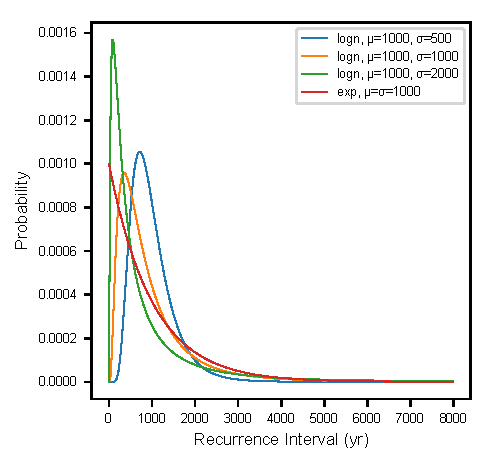
\includegraphics[width=8.3cm]{./figures/recurrence_dists.pdf}
\caption{Earthquake recurrence distributions. `logn' = lognormal. `exp' = 
  exponential. Colors for each distributions are the same in all figures. 
  \label{eq_rec_dists}}
\end{figure}

\clearpage

\begin{figure}[t]
  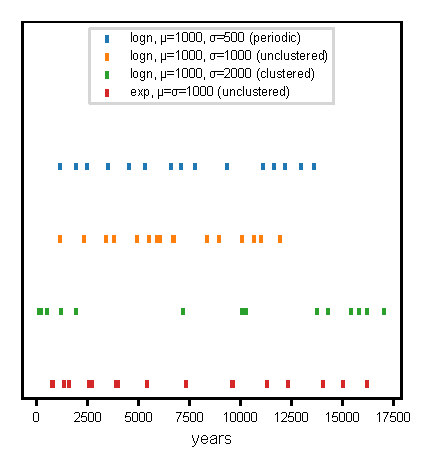
\includegraphics[width=8.3cm]{./figures/event_spacing.pdf}
  \caption{Spacing of 15 simulated successive earthquakes from each recurrence 
  distribution. Note that the gap between the last displayed earthquake and the 
  right side of the plot does not represent a long recurrence interval. 
  \label{eq_spacing}}
\end{figure}

\clearpage

\begin{figure}[t]
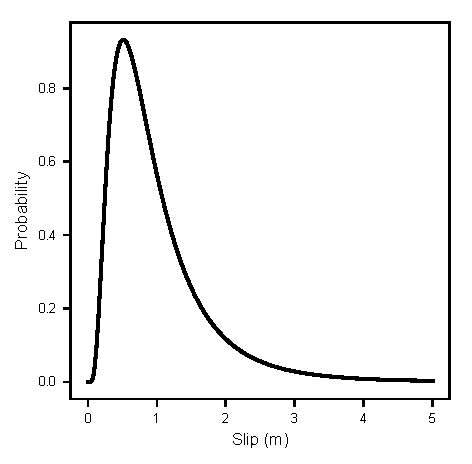
\includegraphics[width=8.3cm]{./figures/slip_dist.pdf}
\caption{Earthquake slip distribution. \label{slip_dist}}
\end{figure}

\clearpage

\begin{figure*}[t]
  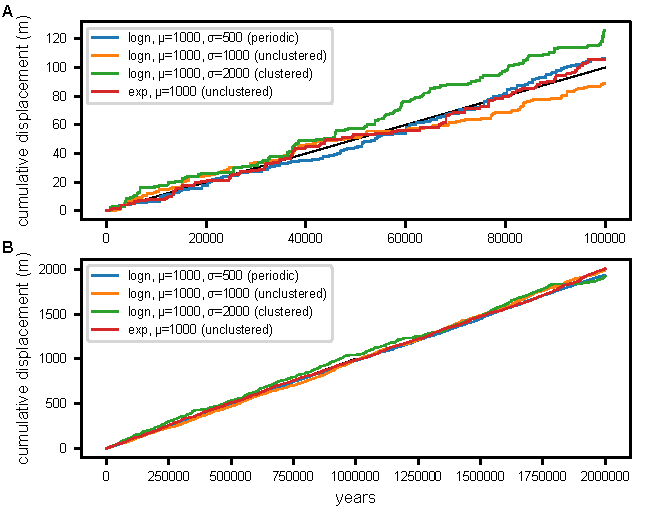
\includegraphics[width=12cm]{./figures/disp_histories.pdf}
  \caption{Simulated displacement histories for each of the recurrence 
  distributions, and the `true' mean line at 1 mm/yr in black. \emph{A}: The 
  first hundred thousand years. \emph{B}: The entire 2 million years. The 
  histories are the same in both plots. \label{disp_histories}}
\end{figure*}


\clearpage


\begin{figure*}[t]
  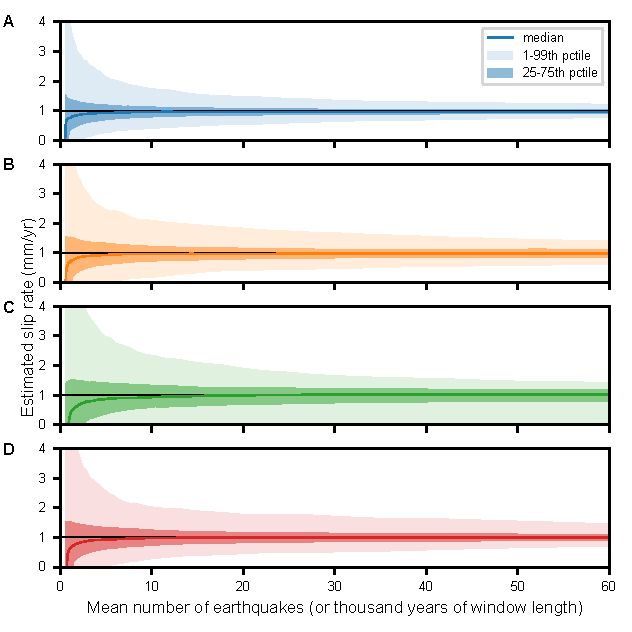
\includegraphics[width=12cm]{./figures/slip_rate_envelopes.pdf}
  \caption{Envelopes of estimated slip rates as a function of the mean number 
  of earthquakes (or thousands of years) over which the slip rate was 
  estimated. All slip rates have a true value of 1 mm/yr. \emph{A}: periodic 
  distribution. \emph{B}: unclustered lognormal distribution. \emph{C}: 
  Clustered lognormal distribution. \emph{C}: Unclustered exponential 
  distribution. \label{slip_rate_envelopes}}
\end{figure*}

\clearpage

\begin{figure*}[t]
  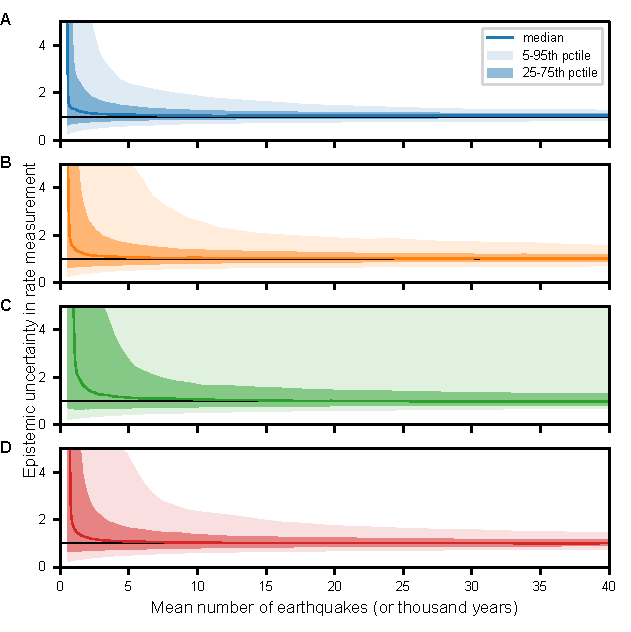
\includegraphics[width=12cm]{./figures/epist_unc.pdf}
  \caption{Epistemic uncertainty relative to the measured rate for each of the 
  recurrence distributions, as a function of the mean number of earthquakes (or 
  thousands of years) over which the slip rates were measured. \emph{A}: 
  periodic distribution. \emph{B}: unclustered lognormal distribution. 
  \emph{C}: Clustered lognormal distribution. \emph{C}: Unclustered exponential 
  distribution.
  \label{epist_unc}}
\end{figure*}

\clearpage

\begin{table}[t]
\begin{tabular}{lllllll}
\tophline
distribution  &  $t$     &     5  &     25 &     50 &    75 &   95 \\
\middlehline
logn\_0.5 & 2531  &  0.51 &  0.79 &  1.13 &  1.77 &  4.37 \\
      & 4843  &  0.61 &  0.84 &  1.08 &  1.46 &  2.44 \\
      & 10,323 &   0.7 &  0.89 &  1.04 &  1.27 &  1.84 \\
      & 42,103 &  0.83 &  0.96 &  1.04 &  1.12 &  1.27 \\
logn\_1 & 2531  &  0.42 &  0.71 &  1.14 &  2.25 &   $\infty$ \\
      & 4843  &  0.51 &  0.75 &  1.07 &  1.67 &  5.62 \\
      & 10,323 &   0.6 &  0.82 &  1.04 &  1.38 &  2.55 \\
      & 42,103 &  0.72 &  0.89 &  1.03 &  1.18 &  1.55 \\
logn\_2 & 2531  &  0.35 &  0.68 &  1.35 &   $\infty$ &   $\infty$ \\
      & 4843  &  0.43 &   0.7 &  1.16 &  2.86 &   $\infty$ \\
      & 10,323 &  0.51 &  0.75 &  1.07 &  1.66 &   $\infty$ \\
      & 42,103 &   0.7 &  0.83 &  0.98 &  1.28 &  4.75 \\
exp\_1 & 2531  &   0.4 &   0.7 &  1.17 &  2.39 &   $\infty$ \\
      & 4843  &  0.49 &  0.75 &  1.08 &  1.67 &  4.79 \\
      & 10,323 &  0.61 &   0.8 &  1.03 &  1.37 &  2.32 \\
      & 42,103 &  0.76 &  0.89 &     1 &  1.15 &  1.43 \\
 \bottomhline
\end{tabular}
  \caption{Epistemic uncertainty table \label{ep_unc_table}}
\end{table}



\end{document}
